% !TeX root =  main.tex

\chapter{Functions}
\thispagestyle{chpg}

\section{Basic Concepts}
\begin{definition}
  A \textbf{relation} is a set of ordered pairs. The set of the first components of each ordered pair is called the \textbf{domain} and the set of the second components of each ordered pair is called the \textbf{range}.

  A \textbf{function} is a relation that assigns each element in the domain a unique element in the range.

  An arbitrary value in the domain is often represented by the lowercase letter $x$ which is called an \textbf{independent variable}.
  An arbitrary output is often represented by the lowercase letter $y$ which is called a \textbf{dependent variable}.
  
  % Each value in the domain is also known as an input value. Each value in the range is also known as an output value.
\end{definition}

\begin{example}
  Determine if the relation 
  \[\{(1,2),(2,4),(3,6),(4,8),(5,10)\}\]
  is a function. Find the domain and the range.
\end{example}

\begin{definition}
  If a function has $x$ as the independent variable and $y$ as the dependent variable, then we often say that $y$ is a function of $x$.
\end{definition}

\begin{example}
  Consider items and prices in a grocery store. Is price a function of item? Is item a function of price? 
\end{example}

\begin{definition}
  A function is often named by letters, such as $f$, $F$, $p$, or $q$. If $f$ is a function of $x$, then we denote it as $y=f(x)$ which is called the \textbf{function notation}. Here $f(x)$ is read as $f$ of $x$ or $f$ at $x$. The notation $f(x)$ represents the output of the function $f$ for a given input $x$.
\end{definition}
  
\begin{example}
  Use function notation to represent a function whose input is the name of a month and output is the number of days in that month.
\end{example}

\newpage


\begin{example}
  A function \(N=f(y)\) gives the number of police officers, \(N\), in a town in year \(y\). What does \(f(2005)=300\) represent?
\end{example}


\begin{example}
  Using a table to represent the days in the month as the function of month.
\end{example}

\begin{example}
  Consider the function $f(x)=x^2+3x-4$. Find the values of the following expressions.

\begin{enumerate}[fourcol]
  \item \(f(2)\)
  \item \(f(a)\)
  \item \(f(a+h)\)
  \item \(\dfrac{f(a+h)-f(a)}{h}\)
\end{enumerate}
\end{example}

\begin{example}
  Consider the function $f(x)=x^2-2x$. Find all $x$ values such that $f(x)=3$.
\end{example}

\newpage

\begin{example}
  Express the relationship defined by the function $2x-y-3=0$ as a function $y=l(x)$.
\end{example}


\begin{example}
  Does the equation \(x^2+y^2=1\) defines $y$ as a function $x$. If so, express the relationship as a function \(y=f(x)\). If not, under what extra condition does the function $y=f(x)$ exist? 
\end{example}


\begin{example}
  Consider the function $f(x)$ defined by a graph below.

  \begin{multicols}{2}
    \begin{enumerate}
      \item Find $f(-1)$. 
      \item Find all $x$ such that $f(x)=3$.
    \end{enumerate}
    \vfill

    \columnbreak
    
    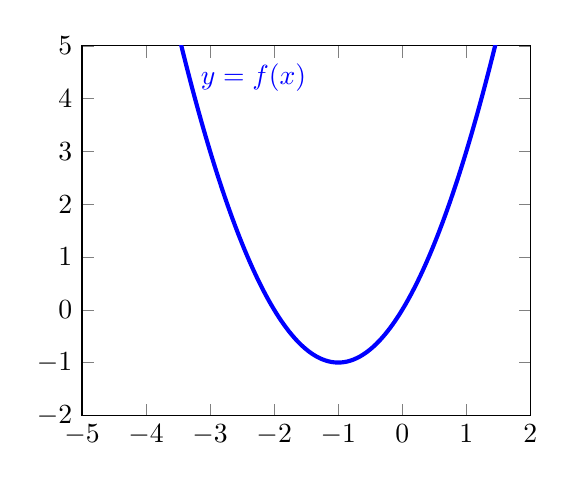
\begin{tikzpicture}
      \begin{axis}[
      width=0.6\textwidth,
      xmin=-5,
      xmax=2,
      ymin=-2,
      ymax=5,
      xtick={-10,-9,...,10},
      ytick={-10,-9,...,10},
      ]
      \addplot[blue, line width=1.5pt, smooth,samples=100] {x^2+2*x} node[pos=0.2, right] {$y=f(x)$};
      \end{axis}
      \end{tikzpicture}

    % \begin{center}
    %   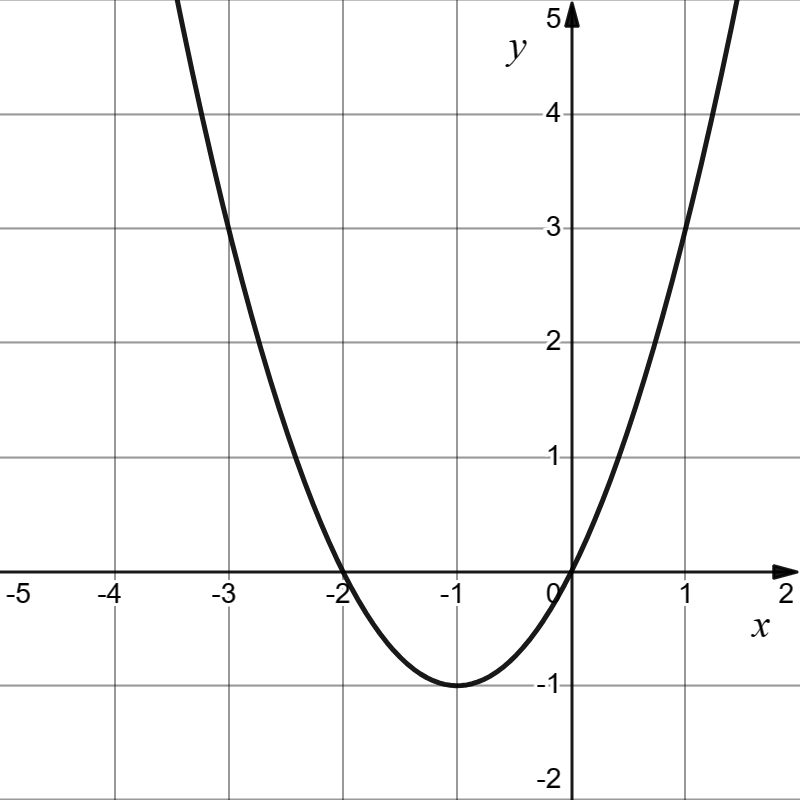
\includegraphics[scale=0.25]{figs/f(x)=x^2+2x.png}
    % \end{center}
  \end{multicols}
\end{example}
\vspace*{-12\baselineskip}

\newpage

\begin{definition}
  A function is a \textbf{one-to-one function} if each output value corresponds to exactly one input value.
\end{definition}

\begin{example}
  Is the area of a circle a function of its radius? If yes, is the function one-to-one?
\end{example}

\begin{howto}
  A graph is a function if very vertical line crosses the graph at most once. This method is known as the \textbf{vertical line test}.

A function is an one-to-one if very horizontal line crosses the graph at most once. This method is known as the \textbf{horizontal line test}.
\end{howto}

\begin{example}
  Determine if the graph defines a function. If so, is it a one-to-one function?
  \begin{center}
  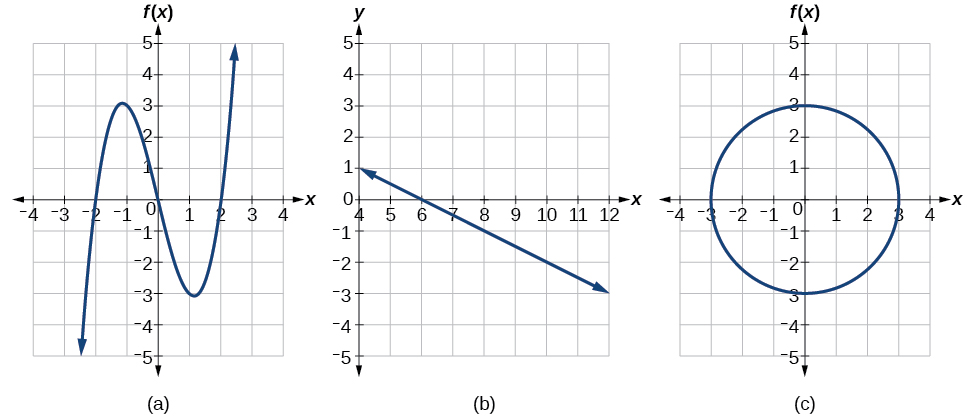
\includegraphics[width=0.8\textwidth]{figs/cubic-line-circle.jpg}
  \end{center}
\end{example}

\newpage
\section*{Exercises}

\begin{exercise}
  Consider the function $f(x)=2x^2+x-3$. Find the values of the following expressions.

\begin{enumerate}[fourcol]
  \item \(f(-1)\)
  \item \(f(a)\)
  \item \(f(a+h)\)
  \item \(\dfrac{f(a+h)-f(a)}{h}\)
\end{enumerate}
\end{exercise}
\vspace*{2\baselineskip}

\begin{exercise}
  For the function $f(x)=-4x+5$, evaluate and simplify the difference quotient $\dfrac{f(x+h)-f(x)}{h}$.
\end{exercise}
\vspace*{2\baselineskip}

\begin{exercise}
  Consider the function $f(x)=-x^2-4x$. Find all $x$ values such that $f(x)=3$.
\end{exercise}

\newpage

\begin{exercise}
  Express the relationship defined by the function $3x-2y-6=0$ as a function $y=l(x)$.
\end{exercise}

\begin{exercise}
  If \(8x-y^3=0\), express \(y\) as a function of \(x\).

  Is $y$ a one-to-one function of $x$?
\end{exercise}


\begin{exercise}
  Consider the function $f(x)$ defined by a graph below.

  \begin{multicols}{2}
    \begin{enumerate}
      \item Find $f(1)$. 
      \item Find all $x$ such that $f(x)=3$.
    \end{enumerate}
    \vfill\mbox{}

    \columnbreak
   
    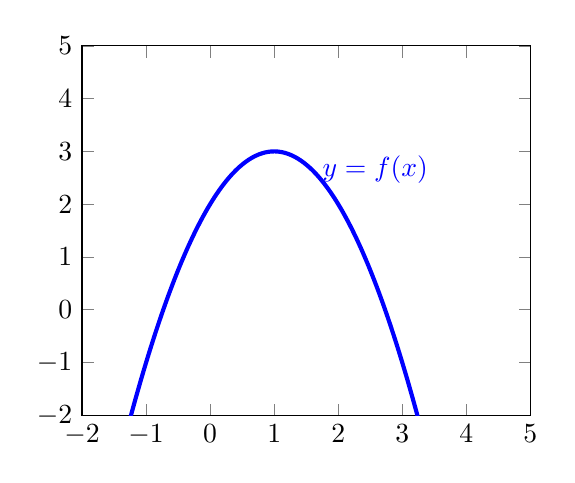
\begin{tikzpicture}
      \begin{axis}[
      width=0.6\textwidth,
      xmin=-2,
      xmax=5,
      ymin=-2,
      ymax=5,
      xtick={-10,-9,...,10},
      ytick={-10,-9,...,10},
      ]
      \addplot[blue, line width=1.5pt, smooth,samples=100] {-x^2+2*x+2} node[pos=0.7, right] {$y=f(x)$};
      \end{axis}
      \end{tikzpicture}

    % \begin{center}
    %   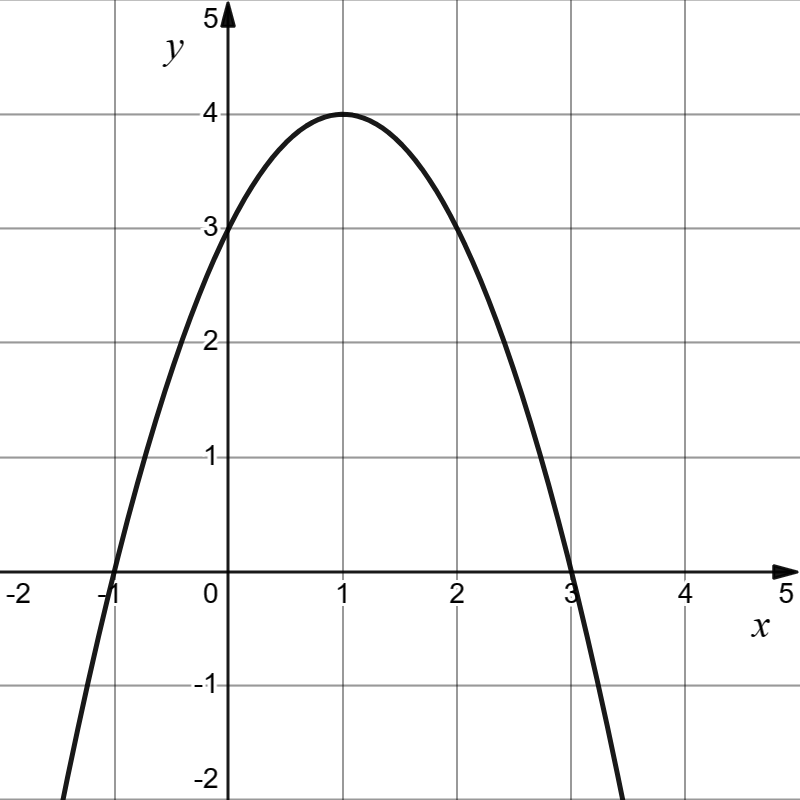
\includegraphics[scale=0.3]{figs/f(x)=-x^2+2x+2.png}
    % \end{center}
  \end{multicols}
\end{exercise}
\vspace{-10\baselineskip}


\newpage
\thispagestyle{fancy}

\section{Domains and Ranges}
\begin{howto}
The domain of a function $f$ consists of possible input values $x$. Or equivalently, the domain consists of all $x$ values except those that will make the function is undefined.

The range of a function $f$ consists of all possible output values $y$. Equivalently, the range consists of $y$ value such that equation $y=f(x)$ has a solution $x$. 
\end{howto}

\begin{example}
  Find the domain of the function $$f(x)=\dfrac{x+1}{2-x}.$$
\end{example}

\begin{example}
  Find the domain of the function
$$
f(x)=\sqrt{7-x}.
$$
\end{example}

\begin{definition}
  \textbf{Set-builder notation} is a method of specifying a set of elements that satisfy a certain condition. It takes the form $\{x|\text{ statement about x}\}$ which is read as, ``the set of all x such that the statement about x is true."
  
  \textbf{Interval notation} is a way of describing sets that include all real numbers between a lower limit that may or may not be included and an upper limit that may or may not be included. The endpoint values are listed between brackets or parentheses. A square bracket indicates inclusion in the set, and a parenthesis indicates exclusion from the set.
\end{definition}

\newpage

\begin{example}
  Find the domain of the function $f(x)=\dfrac{\sqrt{x+2}}{x-1}$. Write your answer in set-builder notation and interval notation.
\end{example}


\begin{example}
  Find the domain and range of the function $f$ whose graph is shown in Figure.

  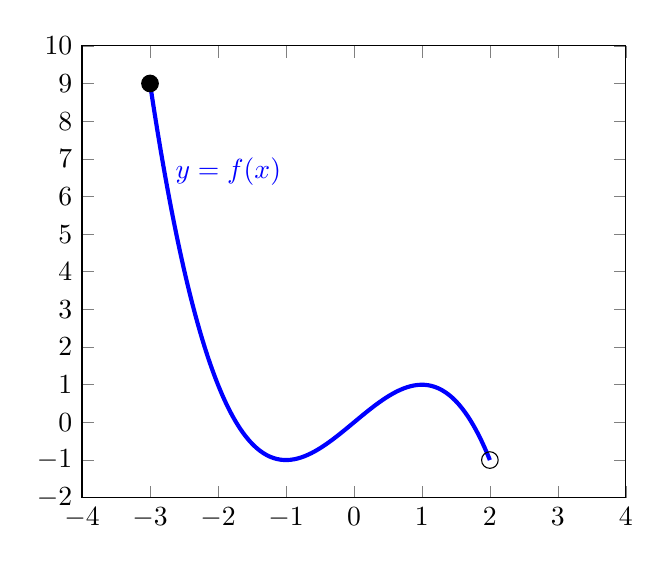
\begin{tikzpicture}
    \begin{axis}[
    width=0.7\textwidth,
    xmin=-4,
    xmax=4,
    ymin=-2,
    ymax=10,
    xtick={-10,-9,...,10},
    ytick={-10,-9,...,10},
    ]
    \addplot[blue, line width=1.5pt, smooth,samples=100,domain=-3:2] {(-x^3+3*x)/2} node[pos=0.15,right] {$y=f(x)$};
    \addplot[mark=*, mark size=3pt] coordinates {(-3,9)};
    \addplot[mark=o, mark size=3pt] coordinates {(2,-1)};
    \end{axis}
    \end{tikzpicture}

  % 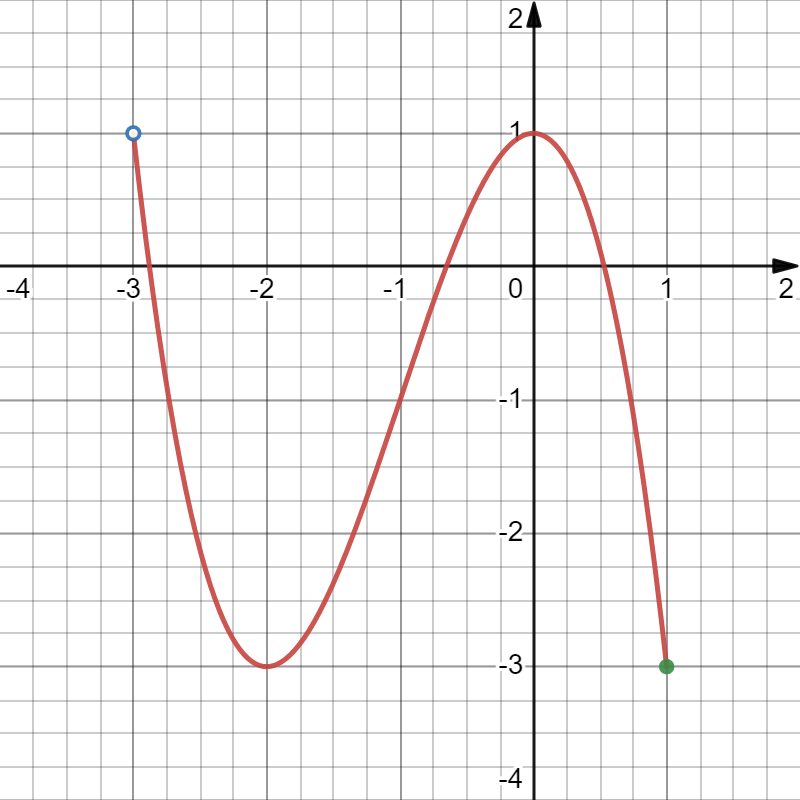
\includegraphics[width=0.6\textwidth]{figs/FindDomainRangeCubic.png}
\end{example}
\vspace*{-8\baselineskip}

\begin{example}
  Find the domain and range of the function
  $$f(x)=\frac{2}{x+3}.$$
\end{example}

\newpage

\begin{example}
  Find the domain and range of the function
  $$f(x)=3\sqrt{x+2}.$$
\end{example}


\begin{example}
  Consider the piecewise function
  $$
  f(x)=\begin{cases}
    2x-3 & \text{if}\quad x\le -1\\
    -x^2 & \text{if}\quad -1<x< 1\\
    -2x+4 & \text{if}\quad 1\le x.
  \end{cases}
  $$
  \begin{enumerate}[threecol]
    \item Sketch the graph
    \item Find $f(-4)$
    \item Find $f(2)$
  \end{enumerate}
\end{example}

\newpage

\section*{Exercises}

\begin{exercise}
  Find the domain of the function\\
  \begin{enumerate*}
    \item  $f(x)=\dfrac{1+4x}{2x-1}$ 
    \item  $f(x)=\sqrt{5+2x}$
    \item  $f(x)=\dfrac{\sqrt{x+1}}{x-1}$
    \item $f(x)=\dfrac{x-2}{x^2+7x-44}$
  \end{enumerate*}
\end{exercise}
\vspace*{\stretch{5}}

\begin{exercise}
  Estimate the domain and range for the function defined by the graph. Write your answer in interval notation.\\
  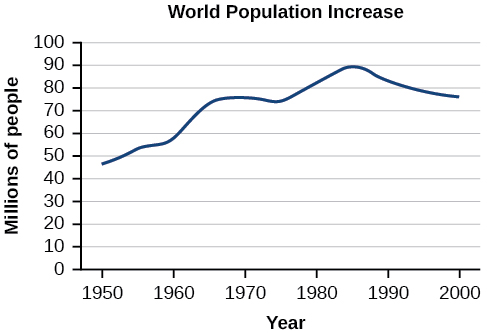
\includegraphics[width=0.6\textwidth]{figs/CNX_Precalc_Figure_01_02_010.jpg}
\end{exercise}
\vspace*{-5\baselineskip}

\newpage

\begin{exercise}
  Find the domain and range of each of the following functions. Write your answer in set-builder notation and interval notation.
  \begin{enumerate}[twocol]
    \item $f(x)=\frac{3}{x-2}$
    \item $f(x)=-2\sqrt{x+4}$
  \end{enumerate}
\end{exercise}

\begin{exercise}
  Consider the piecewise function
  $$f(x)=\begin{cases}
    -2x+5 & \text{if}\quad x< -2\\
    x^2-1 & \text{if}\quad -2\le x\le 2\\
    2x-3 & \text{if}\quad 2< x.
  \end{cases}$$
  \begin{enumerate}[threecol]
    \item Sketch the graph
    \item Find $f(-4)$
    \item Find $f(2)$
  \end{enumerate}
\end{exercise}

\newpage

\section{Rates of Change and Behavior of Graphs}

\begin{definition}[Rate of Change]
  The average rate of change of $f$ over an interval $[a,b]$ is defined as
  $$\text{Average Rate Of Change}=\dfrac{f(b)-f(a)}{b-a}.$$
  The average rate of change is the same as the slope of secant line passing through $(a, f(a))$ and $(b, f(b))$.
  
  By taking $x=a$ and $h=b-a$, the average of rate of change is the same the difference quotient of a function $f$ which is defined as
  $$\text{Difference Quotient}=\dfrac{f(x+h)-f(x)}{h}.$$
\end{definition}

\begin{example}
  After picking up a friend who lives 10 miles away, Anna records her distance from home over time. The values are shown in Table. Find her average speed over the first 6 hours.
\begin{center}
  \begin{tabular}{l*{8}{c}}
    $t$ (hours) & 0 & 1 & 2 & 3 & 4 & 5 & 6 & 7\\
    $D(t)$ (miles) & 10 & 55 & 90 & 153 & 214 & 240 & 292 & 300
  \end{tabular}
\end{center}
\end{example}

\begin{example}
  Find the average rate of change of $f(x)=x^2-\dfrac{1}{x}$ over the interval $[2, 4]$.
\end{example}

\newpage

\begin{example}
  Find the average rate of change of  $g(t)=t^2+3t+1$ on the interval  $[0,a]$. The answer will be an expression involving $a$.
\end{example}



\begin{definition}[Increasing and Decreasing]
  A function $f$ is \textbf{increasing} over an interval $(a, b)$ if $f(x_2)>f(x_1)$ for any $x_1<x_2$ in $(a, b)$. Equivalently, $f$ is increasing over $(a, b)$ if  the average rate of change is positive over any subinterval $(x_1, x_2)$ of $(a, b)$.
  
  A function $f$ is \textbf{decreasing} over an interval $(a, b)$ if $f(x_2)<f(x_1)$ for any $x_1<x_2$ in $(a, b)$. Equivalently, $f$ is decreasing over $(a, b)$ if  the average rate of change is negative over any subinterval $(x_1, x_2)$ of $(a, b)$.

  \begin{center}
    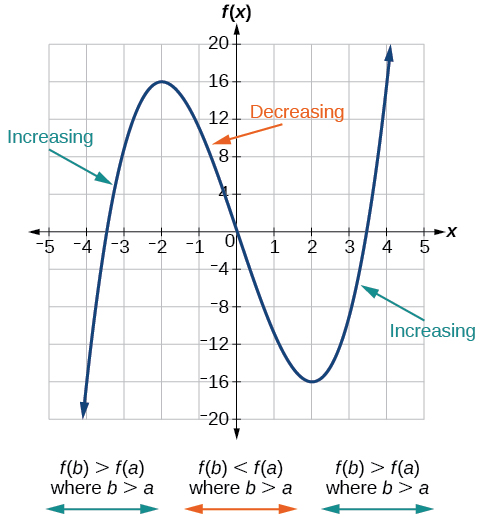
\includegraphics[width=0.6\textwidth]{figs/CNX_Precalc_Figure_01_03_004.jpg}
  \end{center}
\end{definition}

\newpage

\begin{definition}[Local Maxima and Minima]
  A function \(f\) has a \textbf{local maximum} at \(x=c\) if $f(c)\ge f(x)$ for any $x$ in a small interval containing $c$. A small interval containing $c$ is also known as a small \text{neighborhood} of $c$.

  A function \(f\) has a \textbf{local minimum} at \(x=c\) if $f(c)\le f(x)$ for any $x$ in a small interval containing $c$.
\end{definition}

\begin{howto}
  A function $f$ has a local maximum at $x=c$ if it changes from increasing to decreasing at $c$ in a neighborhood of $c$.
  
  A function $f$ has a local minimum at $x=c$ if it changes from decreasing to increasing at $c$ in a neighborhood of $c$.
\end{howto}



\begin{example}
  Find the interval of increasing and the interval of decreasing, and the local maxima and local minima of the function $f$ defined by the following graph.

  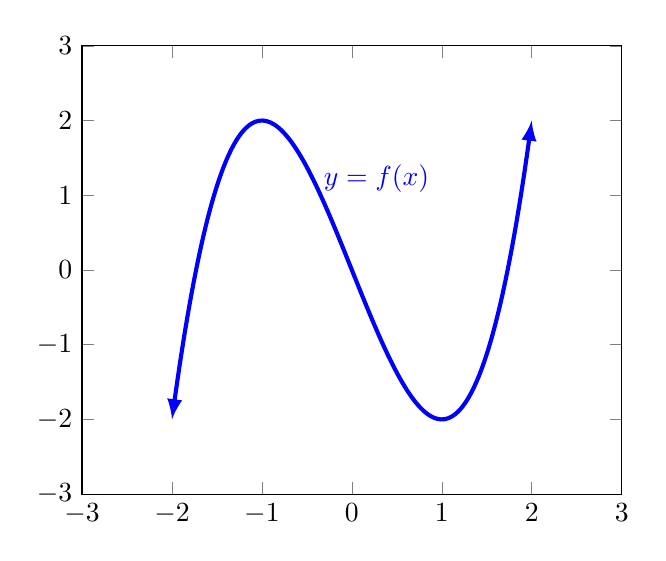
\begin{tikzpicture}
    \begin{axis}[
    xmin=-3,
    xmax=3,
    ymin=-3,
    ymax=3,
    xtick={-10,-9,...,10},
    ytick={-10,-9,...,10},
    ]
    \addplot[latex-latex, blue, line width=1.5pt, smooth,samples=100,domain=-2:2] {x^3-3*x} node[pos=0.4, right] {$y=f(x)$};
    \end{axis}
  \end{tikzpicture}

  % \begin{center}
  %   \raggedright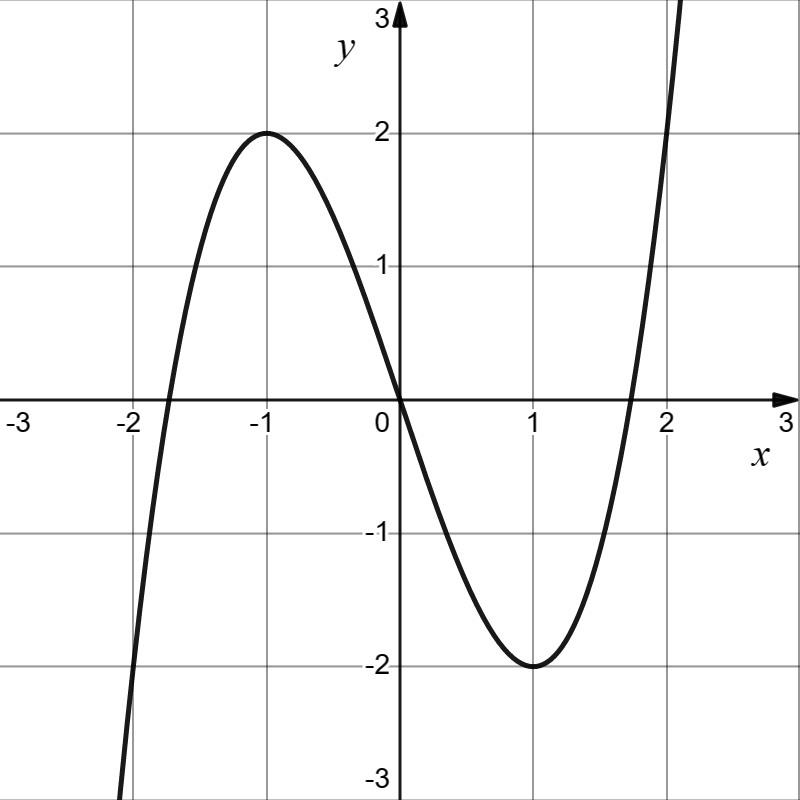
\includegraphics[width=0.5\textwidth]{figs/x^3-3x.png}
  % \end{center}
\end{example}

% \vspace*{-0.1\textheight}
% \newpage

\begin{definition}[Absolute Maxima and Minima]
  The \textbf{absolute maximum} of $f$ at \(x=c\) is \(f(c)\) where \(f(c)\ge f(x)\) for all \(x\) in the domain of \(f\).
  
  The \textbf{absolute minimum} of $f$ at \(x=c\) is \(f(c)\) where \(f(c)\le f(x)\) for all \(x\) in the domain of \(f\).
\end{definition}

\begin{example}
  Finding the absolute maximum and minimum of the function $f$ defined by the following graph.
  
  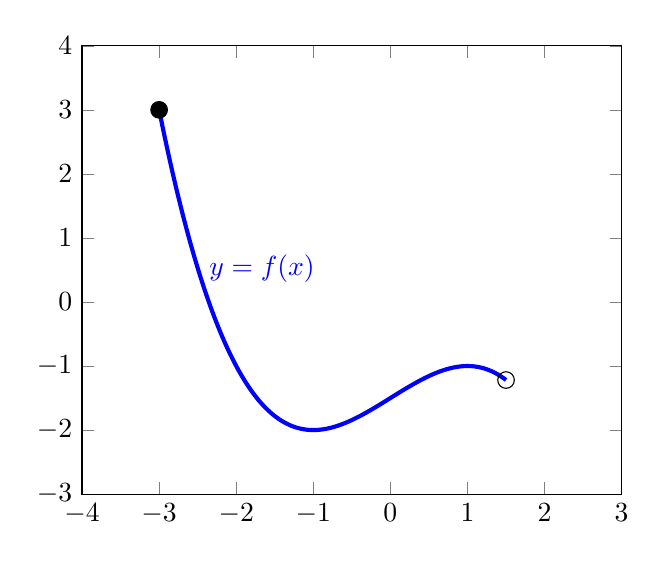
\begin{tikzpicture}
    \begin{axis}[
    % width=0.6\textwidth,
    xmin=-4,
    xmax=3,
    ymin=-3,
    ymax=4,
    xtick={-10,-9,...,10},
    ytick={-10,-9,...,10},
    ]
    \addplot[blue, line width=1.5pt, smooth,samples=100,domain=-3:1.5] {(-x^3+3*x-6)/4} node[pos=0.3, right] {$y=f(x)$};
    \addplot[mark=*, mark size=3pt] coordinates {(-3,3)};
    \addplot[mark=o, mark size=3pt] coordinates {(1.5,-1.21875)};
    \end{axis}
    \end{tikzpicture}

  % \begin{center}
  %   \raggedright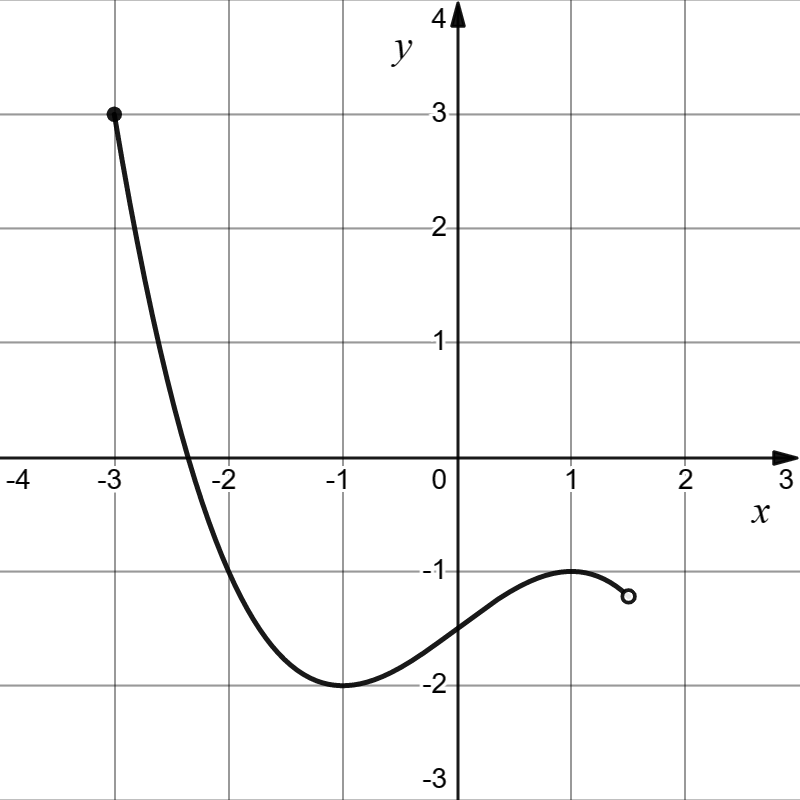
\includegraphics[width=0.5\textwidth]{figs/(-x^3+3x-6)divby4.png}
  % \end{center}
\end{example}

\newpage
\section*{Exercises}

\begin{exercise}
  The electrostatic force  $F$, measured in newtons, between two charged particles can be related to the distance between the particles  $d$, in centimeters, by the formula  $F(d)=\dfrac{2}{d^2}$. Find the average rate of change of force if the distance between the particles is increased from 2 cm to 6 cm.
\end{exercise}

\begin{exercise}
  Find the average rate of change of $f(x)=x^2+2x-8$ on the interval $[5,a]$.
\end{exercise}

\begin{exercise}
  Find the interval of increasing and the interval of decreasing, and the local maxima and local minima of the function $f$ defined by the following graph.

  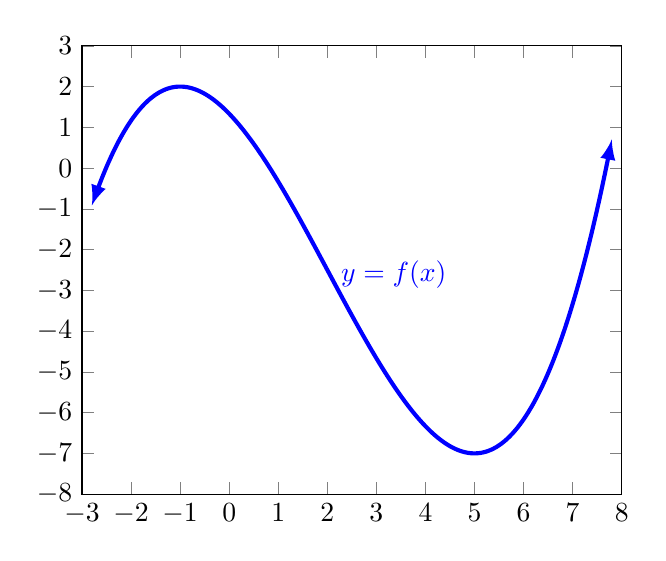
\begin{tikzpicture}
    \begin{axis}[
    xmin=-3,
    xmax=8,
    ymin=-8,
    ymax=3,
    xtick={-10,-9,...,10},
    ytick={-10,-9,...,10},
    ]
    \addplot[latex-latex, blue, line width=1.5pt, smooth,samples=100,domain=-2.8:7.8] {(x^3-6*x^2-15*x+16)/12} node[pos=0.4, right] {$y=f(x)$};
    \end{axis}
    \end{tikzpicture}
  % \begin{center}
  %   \raggedright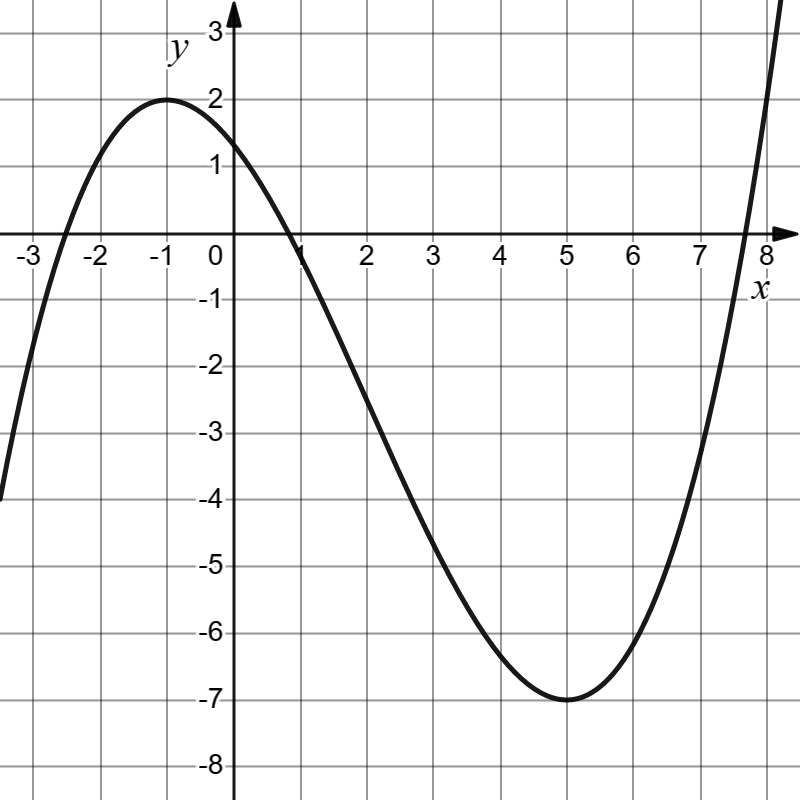
\includegraphics[width=0.5\textwidth]{figs/(xcube-6xsq-15x+16)divby12.png}
  % \end{center}
\end{exercise}
\vspace{-12\baselineskip}

\newpage

\begin{exercise}
  Finding the absolute maximum and minimum of the function $f$ defined by the following graph.
  
  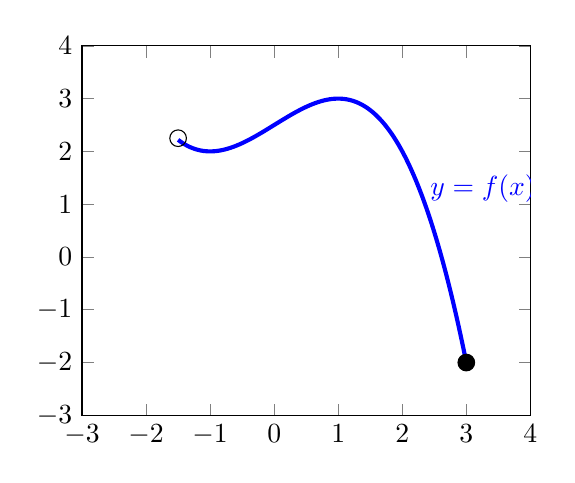
\begin{tikzpicture}
    \begin{axis}[
    width=0.6\textwidth,
    xmin=-3,
    xmax=4,
    ymin=-3,
    ymax=4,
    xtick={-10,-9,...,10},
    ytick={-10,-9,...,10},
    ]
    \addplot[blue, line width=1.5pt, smooth,samples=100,domain=-1.5:3] {(-x^3+3*x+10)/4} node[pos=0.6, right] {$y=f(x)$};
    \addplot[mark=*, mark size=3pt] coordinates {(3,-2)};
    \addplot[mark=o, mark size=3pt] coordinates {(-1.5,2.25)};
    \end{axis}
    \end{tikzpicture}

  % \begin{center}
  %   \raggedright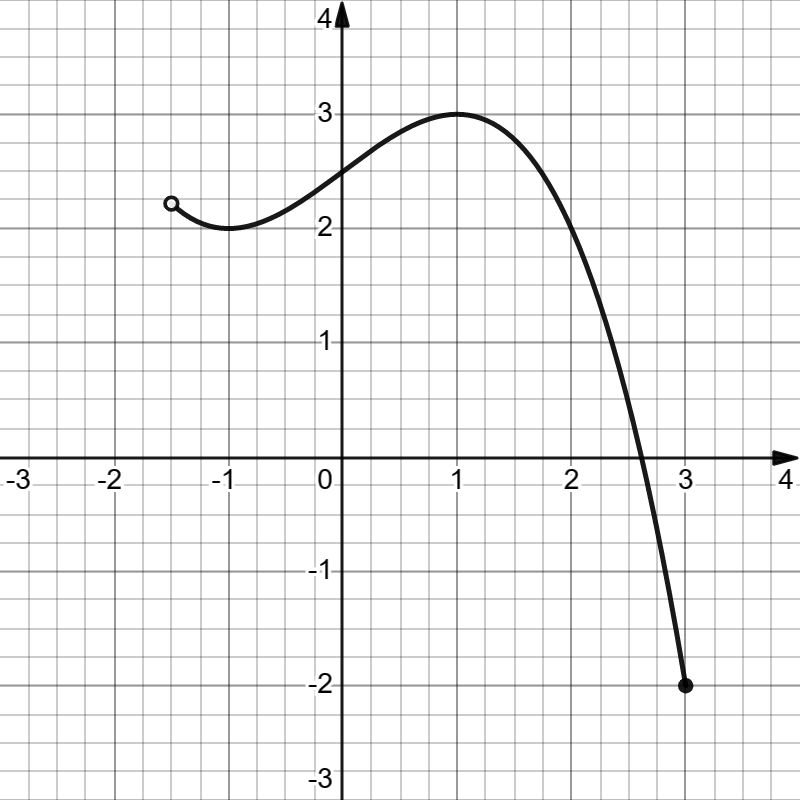
\includegraphics[width=0.5\textwidth]{figs/(-x^3+3x+10)divby4.png}
  % \end{center}
\end{exercise}
\vspace*{-0.4\textheight}

\begin{exercise}
  Find the interval of increasing and the interval of decreasing, and the local maxima and local minima of the function $f(x)=x^3-6x^2-15x+20$ using its graph.
  %f\left(x\right)=2x^{3}-3x^{2}-12x+7
\end{exercise}

\newpage

\section{Combination and Composition of Functions}

\begin{definition}[Algebraic Operations of Functions]
  Let \(f\) and \(g\) be two functions with domains $A$ and $B$ respectively. We define the linear combination, product, and quotient functions as follows.
  \begin{center}
    \begin{tabular}{rcl}
      Linear combination: & $(af+bg)(x)=af(x)+bg(x)$ & with the domain $A\cap B$.\\
      Product: & $(fg)(x)=f(x)g(x)$ & with the domain: $A\cap B$.\\
      Quotient: & $\left(\dfrac{f}{g}\right)(x)=\dfrac{f(x)}{g(x)}$ & with the domain: $A\cap B\cap \{x\mid g(x)\neq 0\}$.
    \end{tabular}
  \end{center}
  
\end{definition}

\begin{example}
  Consider the functions \(f(x)=x-1\) and \(g(x)=x^2-1\). Find and simplify the functions \((g-f)(x)\) and \(\left(\dfrac{g}{f}\right)(x)\), and their domains.
\end{example}

\begin{definition}[Composition of functions]
  Let \(f\) and \(g\) be two functions with domains $A$ and $B$ respectively. The \textbf{composite function} $f\circ g$ (also called the
  composition of $f$ and $g$) is defined as
  \[(f\circ g)(x)=f(g(x))\qquad \text{with the domain:}\quad B\cap \{x\mid g(x)\in A\}.\]
\noindent
  We read the left-hand side as ``\(f\) composed with \(g\) at \(x\),'' and the right-hand side as ``\(f\) of \(g\) of \(x\).''
\end{definition}

\begin{example}
  Consider the functions \(f(x)=\sqrt{x-2}\) and \(g(x)=x^2+1\). 
  \begin{enumerate}
    \item Find and simplify the functions \((f\circ g)(x)\) and \((g\circ f))(x)\).  Are they the same function?
    \item Find the domains of $f\circ g$ and $g\circ f$. Are they the same?
  \end{enumerate}
\end{example}

\newpage

\begin{example}
  Consider $f(t)=t^2-4t$ and $h(x)=\sqrt{x+3}$. Evaluate\\ 
  \begin{enumerate*}
    \item $\dfrac{f(1)}{g(1)}$
    \item $h(f(-1))$
    \item $(f\circ h)(-1))$
    \item $(f-h)(-1)$
  \end{enumerate*}
\end{example}

\vspace*{2\baselineskip}

\begin{example}
  Using the graphs to evaluate the given functions.
  \begin{multicols}{2}
    \begin{enumerate}
      \item $(f+g)(1)$
      \item $(fg)(1)$
      \item $\left(\dfrac{f}{g}\right)(1)$
      \item $(g\circ f)(-3)$
      \item $f(g(0))$
      % \vfill\mbox{}
    \end{enumerate}
    \columnbreak
    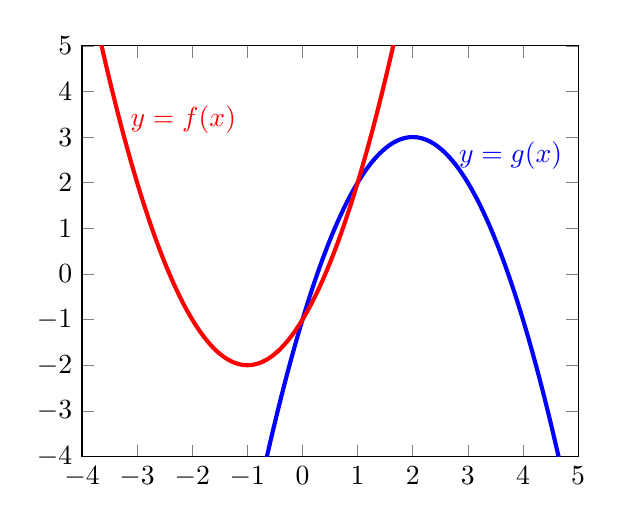
\begin{tikzpicture}
      \begin{axis}[
        width=0.65\textwidth,
      xmin=-4,
      xmax=5,
      ymin=-4,
      ymax=5,
      xtick={-10,-9,...,10},
      ytick={-10,-9,...,10},]
      \addplot[blue, line width=1.5pt, smooth,samples=100] {-(x-2)^2+3} node[pos=0.85, right] {$y=g(x)$};
      \addplot[red, line width=1.5pt, smooth,samples=100] {(x+1)^2-2} node[pos=0.2, right] {$y=f(x)$};
      \end{axis}
      \end{tikzpicture}

    % 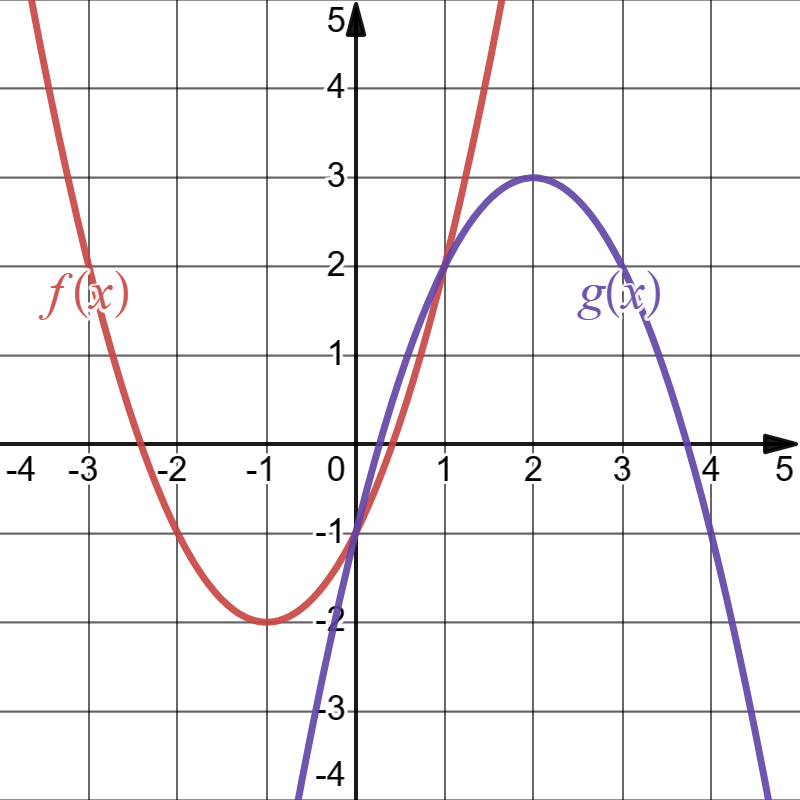
\includegraphics[width=0.45\textwidth]{figs/twoquadratics.png}
  \end{multicols}
\end{example}
\vspace*{-0.1\textheight}

\begin{example}
  Consider the function $h(x)=\sqrt{x^2+1}$. Find two functions $f$ and $g$ so that $h(x)=f(g(x))$.
\end{example}

\newpage

\section*{Exercises}

\begin{exercise}
  Consider the functions \(f(x)=x^2-1\) and \(g(x)=x+1\). 
  \begin{enumerate}
    \item Find the function \((f-g)(x)\) and its domain.
    \item Find the function \((fg)(x)\) and its domain.
    \item Find \(\left(\dfrac{f}{g}\right)(x)\) and its domain.
    \item Find \((2f-3g)(1)\).
    \item Find \(2fg-\left(\dfrac{3g}{f}\right)(1)\).
  \end{enumerate}
\end{exercise}

\begin{exercise}
  Consider the functions $f(x)=\dfrac{1}{x-2}$ and $g(x)=\sqrt{x+4}$.

\begin{enumerate}
  \item Find $f\circ g$ and its domain.
  \item Find $(g\circ f)(3)$.
\end{enumerate}
\end{exercise}

\newpage

\begin{exercise}
    Using the graphs to evaluate the given functions.
    \begin{multicols}{2}
      \begin{enumerate}
        \item $(f-g)(1)$
        \item $(fg)(0)$
        \item $\left(\dfrac{f}{g}\right)(0)$
        \item $(f\circ g)(2)$
        \item $g(f(0))$
      \end{enumerate}

      \columnbreak

      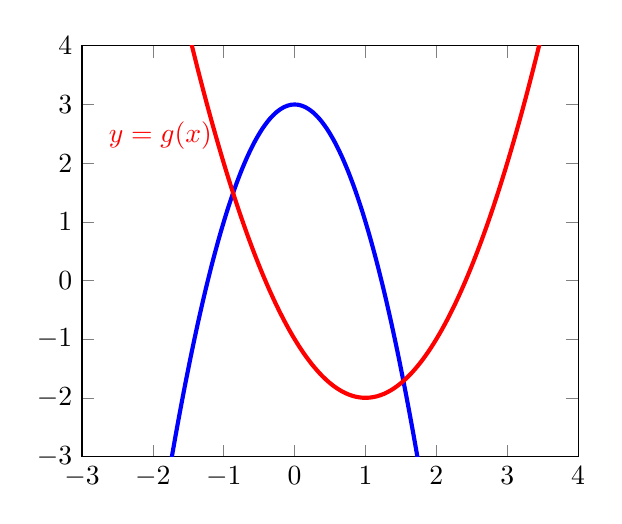
\begin{tikzpicture}
        \begin{axis}[
          width=0.65\textwidth,
        xmin=-3,
        xmax=4,
        ymin=-3,
        ymax=4,
        xtick={-10,-9,...,10},
        ytick={-10,-9,...,10},]
        \addplot[blue, line width=1.5pt, smooth,samples=100] {-2*x^2+3} node[pos=0.6, above right] {$y=f(x)$};
        \addplot[red, line width=1.5pt, smooth,samples=100] {(x-1)^2-2} node[pos=0.6, above left] {$y=g(x)$};
        \end{axis}
        \end{tikzpicture}

      % 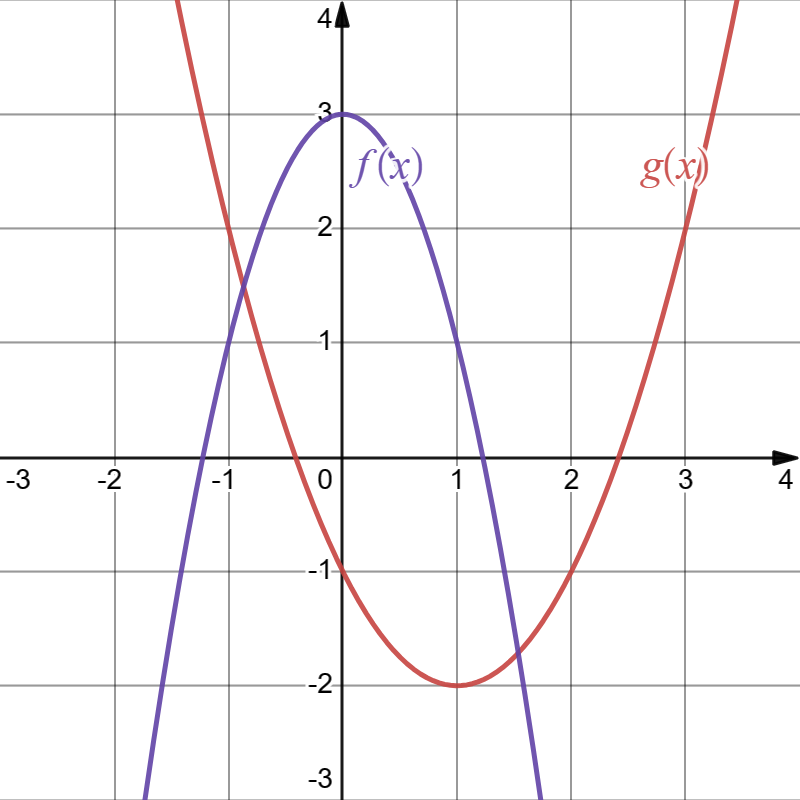
\includegraphics[width=0.5\textwidth]{figs/two-quadratics-exr.png}
    \end{multicols}
\end{exercise}
\vspace*{-0.2\textheight}

\begin{exercise}
  Consider the function $h(x)=\sqrt[3]{2x-1}$. Find two functions $f$ and $g$ so that $h(x)=f(g(x))$.
\end{exercise}

\newpage

\section{Transformations}

\begin{definition}
  A function $y=g(x)$ that is obtained by substituting $x$ by $Bx-C$ and substituting $y$ by $Ay-D$, where $AB\ne 0$, from a function $y=f(x)$, is called a transformation of $f$.
  
  \begin{enumerate}
    \item If $A=B=1$ and $C=0$, $g$ is called a vertical shift of $f$ by $C$ units.
    \item If $A=B=1$ and $D=0$, $g$ is called a horizontal shift of $f$ by $D$ units.
    \item If $A=1$, $B=-1$ and $C=D=0$, $g$ is called a horizontal reflection or a reflection along the $y$-axis of $f$.
    \item If $A=-1$, $B=1$ and $C=D=0$, $g$ is called a vertical reflection or a reflection along the $y$-axis of $f$.
    \item If $A=1$ and $C=D=0$, $g$ is called a horizontal stretch or compression of $f$ by a factor $\dfrac{1}{B}$ if $0<B<1$ or $B>1$ respectively.
    \item If $B=1$ and $C=D=0$, $g$ is called a vertical stretch or compression of $f$ by a factor $\dfrac{1}{A}$ if $0<A<1$ or $A>1$ respectively.
  \end{enumerate}
\end{definition}


\begin{example}
  Consider the functions $f(x)=x^2$, $g(x)=x^2-1$ and $h(x)=x^2+2$.
  \begin{enumerate}
    \item Describe how to get the graph of $g$ from the graph of $f$.
    \vspace*{3\baselineskip}
    \item Describe how to get the graph of $h$ from the graph of $f$.
    \vspace*{3\baselineskip}
    \item Describe how to get the graph of $f$ from the graph of $h$.
    \vspace*{3\baselineskip}
    \item Describe how to get the graph of $h$ from the graph of $g$.
    \vspace*{3\baselineskip}
  \end{enumerate}
\end{example}

\begin{example}
  Consider the functions $f(x)=x^2$, $g(x)=(x+1)^2$ and $h(x)=(x-2)^2$.
  \begin{enumerate}
    \item Describe how to get the graph of $g$ from the graph of $f$.
    \vspace*{3\baselineskip}
    \item Describe how to get the graph of $h$ from the graph of $f$.
    \vspace*{3\baselineskip}
    \item Describe how to get the graph of $f$ from the graph of $h$.
    \vspace*{3\baselineskip}
    \item Describe how to get the graph of $h$ from the graph of $g$.
    \vspace*{3\baselineskip}
  \end{enumerate}
\end{example}

\newpage

\begin{example}
  Sketch the graph of \(f(x)=|x|\) and then use the graph to sketch the graph of \(h(x)=f(x+2)-1\). 
\end{example}

\begin{example}
  The function $y=g(x)$ shown in the picture is a shift of the square root function $y=\sqrt{x}$. Find $g(x)$.\\

  \begin{tikzpicture}[scale=1.2]
    \begin{axis}[
    xmin=-2,
    xmax=2,
    ymin=-2,
    ymax=2,
    xtick={-5,-4,...,5},
    ytick={-5,-4,...,5},]
    \addplot[blue, line width=1.5pt, smooth,samples=100,domain=-1:2] {sqrt(x+1)-1} node[pos=0.7, above left] {$y=g(x)$};
    \end{axis}
    \end{tikzpicture}
\end{example}
\vspace*{-0.4\textheight}

\newpage

\begin{example}
  Reflect the graph of \(f(x)=|x-1|\)\\
  \begin{enumerate*}
    \item first vertically,
    \item then horizontally.\hfill\mbox{}
  \end{enumerate*}

Denote the new function by $y=g(x)$. Find $g(x)$.
\end{example}

\begin{example}
  A common model for learning has an equation similar to \(k(t)=-2^{-t}+1\), where \(k\) is the percentage of mastery that can be achieved after \(t\) practice sessions, and $t>0$. The function $k$ is a transformation of a part of the function \(f(t)=2^t\) shown below. Sketch the graph of \(k(t)\).\\
  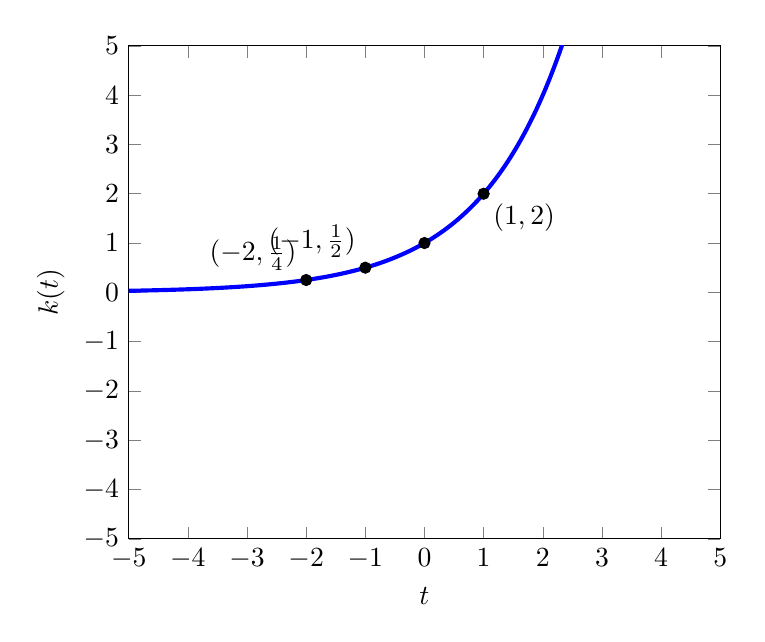
\begin{tikzpicture}
    \begin{axis}[
      width=0.75\textwidth,
    xmin=-5,
    xmax=5,
    ymin=-5,
    ymax=5,
    xlabel={$t$},
    ylabel={$k(t)$},
    xtick={-10,-9,...,10},
    ytick={-10,-9,...,10},]
    \addplot[blue, line width=1.5pt, smooth,samples=100,domain=-5:3] {2^x} node[pos=0.9, right] {$y=f(x)$};
    \addplot[mark=*] coordinates {(-2, 0.25)} node[above left] {$(-2,\frac14)$};
    \addplot[mark=*] coordinates {(-1, 0.5)} node[above left] {$(-1,\frac12)$};
    \addplot[mark=*] coordinates {(0, 1)};
    \addplot[mark=*] coordinates {(1, 2)} node[below right] {$(1,2)$};
    \end{axis}
    \end{tikzpicture}

% 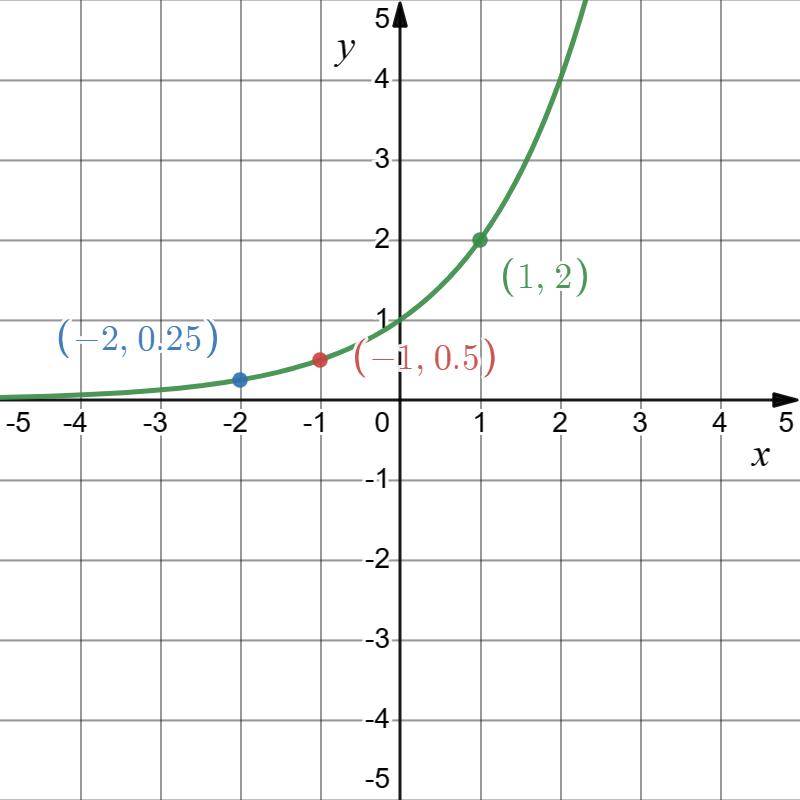
\includegraphics[width=0.5\textwidth]{figs/learningmodel.png}
\end{example}
\vspace*{-0.3\textheight}



\begin{example}
  The point $(9, -15)$ is on the graph of $y=f(x)$. Find a point on the graph of $g(x)=\dfrac{1}{3}f(x)$.
\end{example}
\vspace*{-0.3\textheight}

\newpage
\begin{example}
  The function $y=g(x)$ given in the following graph can be obtained from $f(x)=x^2$ by a combination of shifting, reflecting, and stretching. Describe the transformation and find an equation of $g$.\\
  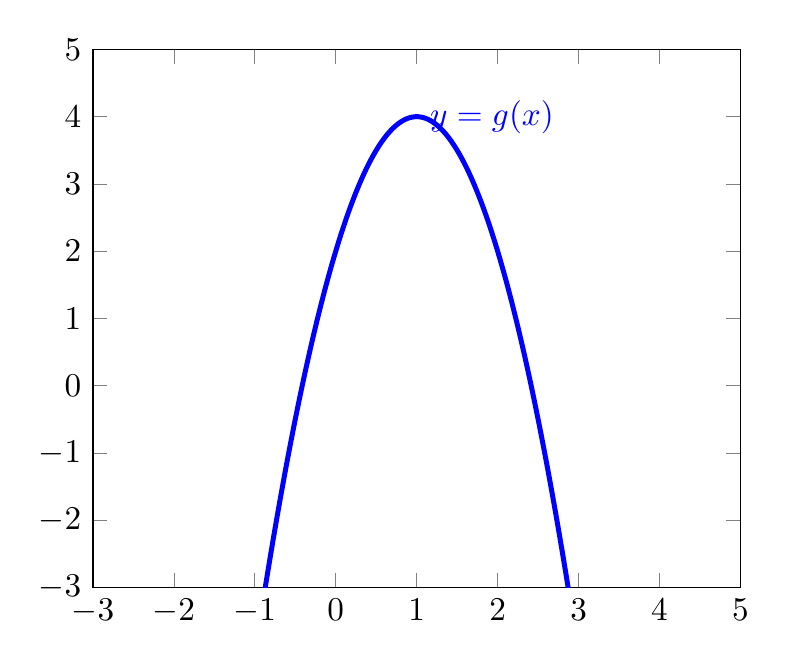
\begin{tikzpicture}[scale=1.2]
    \begin{axis}[
    xmin=-3,
    xmax=5,
    ymin=-3,
    ymax=5,
    xtick={-10,-9,...,10},
    ytick={-6,-5,...,6},]
    \addplot[blue, line width=1.5pt, smooth,samples=100,domain=-1:3] {-2*(x-1)^2+4} node[pos=0.5, right] {$y=g(x)$};
    \end{axis}
    \end{tikzpicture}

  % 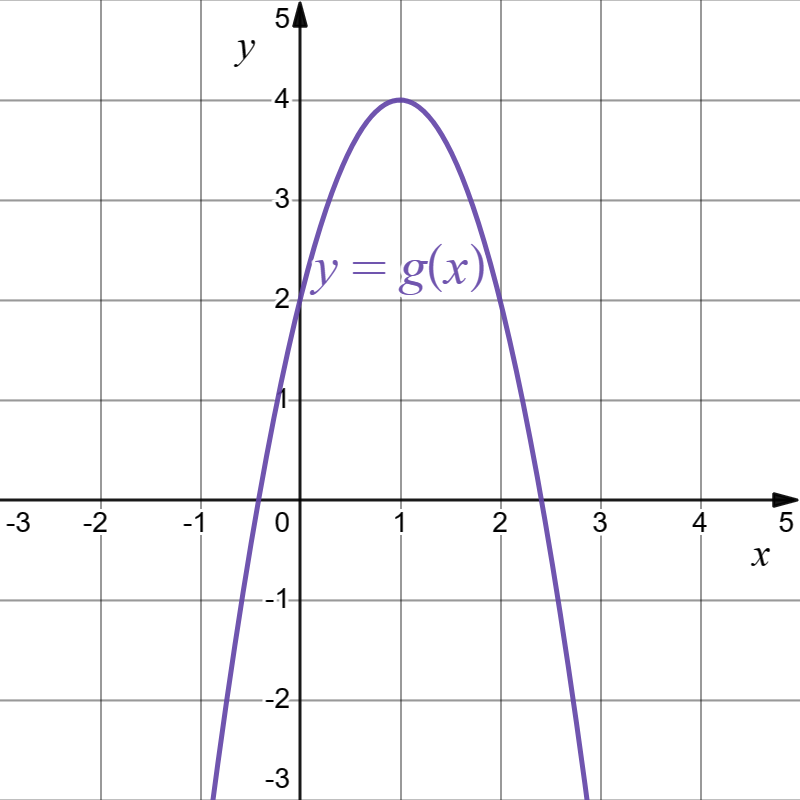
\includegraphics[width=0.5\textwidth]{figs/transformationquadratic.png}
\end{example}
\vspace*{-0.1\textheight}

\begin{example}
  The function $y=f(x)$ has two $x$-intercepts $(-2, 0)$ and $(4, 0)$. Determine if the function $g(x)=f(2x)$ has any $x$-intercepts. If so, find them. Otherwise explain why it has no $x$-intercept.
\end{example}

\begin{example}
  Describe how to get the graph of the function $g(x)=4x^2$ from the graph of the function $f(x)$.
\end{example}
\newpage

\begin{example}
  Using the graph of the function $y=f(x)$ given below to sketch the graph of the function $g(x)=-2f(3x-6)+4$.\\
  \begin{tikzpicture}[scale=1.2]
    \begin{axis}[
    xmin=-3,
    xmax=3,
    ymin=-2,
    ymax=4,
    xtick={-10,-9,...,10},
    ytick={-6,-5,...,6},]
    \addplot[blue, line width=1.5pt, smooth,samples=100,domain=-2:2] {-abs(x)+2} node[pos=0.5, above right] {$y=f(x)$};
    \end{axis}
    \end{tikzpicture}

  % 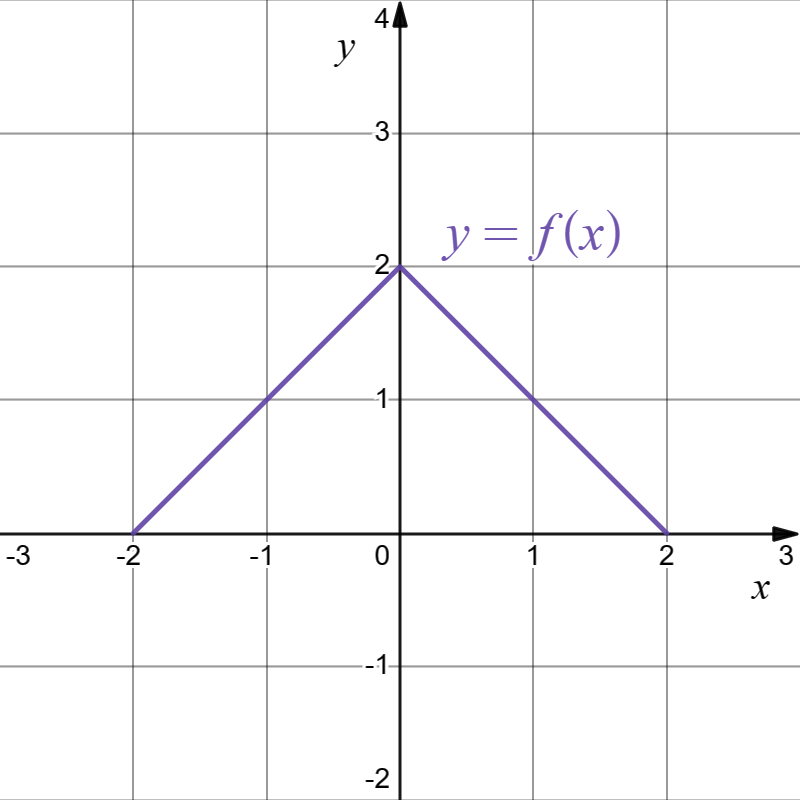
\includegraphics[width=0.5\textwidth]{figs/-abs(x)+2.png}
\end{example}

\newpage

\begin{example}
Sketch the graph of the function $g(x)=2\sqrt{3x-1}-4$ by a sequence of transformation applied on the graph of $f(x)=\sqrt{x}$.  
\end{example}

\begin{example}
  Find an equation of the function $y=g(x)$ whose graph is obtained from $f(x)=\sqrt{x}$ by the following transformations in the given order.
  \begin{enumerate}
    \item stretch vertically by a factor of 2
    \item shift downward 2 units
    \item shift 3 units to the left
    \item stretch vertically by a factor $\dfrac{1}{2}$.
  \end{enumerate}
\end{example}

\newpage

\begin{definition}
  A function is called an \textbf{even function} if $f(-x)=f(x)$ for $x$ in the domain of $f$.
  
  A function is called an \textbf{odd function} if $f(-x)=-f(x)$ for $x$ in the domain of $f$.
\end{definition}

\begin{remark}
  The graph of an even function is symmetric about $y$-axis.

  The graph of an odd function is symmetric about the origin. This symmetry is known as a rotation symmetry.
\end{remark}

\begin{example}
  Group the functions according to even, odd, or other.\\
  \begin{enumerate*}
    \item $f(x)=x^2-1$
    \item $g(x)=|x-1|$
    \item $h(x)=x^3-2x$
    \item $k(x)=\dfrac{1}{x^2}$.
  \end{enumerate*}
\end{example}


\newpage

\section*{Exercises}

\begin{exercise}
    Consider the functions $f(x)=x^2$, $g(x)=(x+1)^2-2$ and $h(x)=(x-2)^2+1$.
    \begin{enumerate}
      \item Describe how to get the graph of $g$ from the graph of $f$.
      \item Describe how to get the graph of $h$ from the graph of $g$.
    \end{enumerate}
\end{exercise}

\begin{exercise}
    Determine if the function is even, odd, or neither.\\
    \begin{enumerate*}
      \item $f(x)=1-x^2$.
      \item $g(x)=\sqrt[3]{-x}$.
      \item $g(x)=x^4-x^3$.
      \hfill\mbox{}
    \end{enumerate*}  
\end{exercise}

\newpage

\begin{exercise}
  Sketch the graph of the function $g(x)=2|3x-6| + 4$ by a sequence of transformation applied on the graph of $f(x)=|x|$.  
\end{exercise}

\begin{exercise}
  Find an equation of the function $y=g(x)$ whose graph is obtained from $f(x)=\sqrt[3]{x}$ by the following transformations in the given order.
  \begin{enumerate}
    \item Compress vertically by a factor of $\dfrac{1}{2}$.
    \item Reflect vertically.
    \item shift downward 2 units.
    \item Compress horizontal by a factor $2$.
    \item Shift 3 units to the right.
  \end{enumerate}
\end{exercise}

\newpage

\section{Inverse Functions}

\begin{definition}
  Let $y=f(x)$ be a one-to-one function with the domain $A$. A function \(f^{-1}(x)\) is an \textbf{inverse function} of \(f\) if \(f^{-1}(f(x))=x\) for all \(x\) in $A$.

The notation \(f^{-1}\) is read “\(f\) inverse.” 
\end{definition}
\begin{remark}
  \begin{enumerate}[series=PropertiesInverse]
    \item If $f$ is a one-to-one function, then it has a unique inverse function $f^{-1}$. Here is the proof. Suppose $g$ is also an inverse $f$. Then $f(g(x))=x=f(f^{-1}(x))$. Then $g(x)=f^{-1}(f(g(x)))=f^{-1}(f(f^{-1}(x)))=f^{-1}(x)$.
    \item Note that if $f^{-1}$ is the inverse of $f$, then $f$ is also the inverse of $f^{-1}$ that is $f(f^{-1})(x)=x$ for all $x$ in the domain of $f^{-1}$.
  \end{enumerate}
  \begin{multicols}{2}
    \begin{enumerate}[resume=PropertiesInverse]
      \item In general, $f^{-1}(x)\neq f(x)^{-1}$.
      \item The graphs of a one-to-one function $f$ and its inverse $f^{-1}$ are symmetric about the diagonal line $y=x$.\\
      \item Suppose $f$ has the domain $A$ and the range $B$, then $f^{-1}$ has the domain $B$ and the range $B$ (and vice verse).
      \vfill\null
    \end{enumerate}
    \columnbreak
\begin{center}
  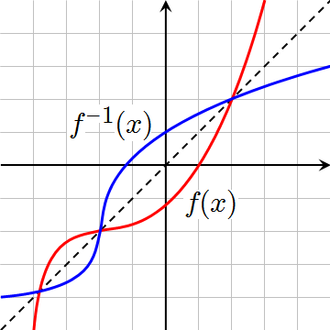
\includegraphics[width=0.25\textwidth]{figs/Inverse_Function_Graph.png}\\
 {\footnotesize The above graph of $f$ and $f^{-1}$ is taken from \href{https://en.wikipedia.org/wiki/Inverse_function}{Wikipedia}.}
\end{center}
\end{multicols}
\end{remark}

\begin{example}
  Let $f$ be a one-to-one function with \(f(3)=4\) and \(f(4)=5\). Find $f^{-1}(4)$.
\end{example}

\begin{example}
  Let $f(x)=\dfrac{1}{x-1}$ and $g(x)=\dfrac{x+1}{x}$. Determine if $g$ is the inverse function of $f$.
\end{example}


\newpage

\begin{example}
  Consider the function $f(x)=x^2+1$ with $x>0$. Sketch the graph of $y=f^{-1}(x)$ without finding its equation.
\end{example}

\begin{howto}
  Given a function $y=f(x)$, the inverse function is the solution $y$ of the equation $f(y)=x$. The domain and the range of $f$ and $f^{-1}$ can be obtained from the domains of $f$ and $f^{-1}$.
\end{howto}


\begin{example}
  Consider the function $f(x)=2x-3$. Find the inverse function $f^{-1}$ and its domain and range.
\end{example}

\begin{example}
  Consider the function $f(x)=\dfrac{x}{x-1}$. Find the inverse function $f^{-1}$ and its domain and range.
\end{example}

\newpage

\begin{example}
  Consider the function $f(x)=2(x+1)^3-1$. Find the inverse function $f^{-1}$ and its domain and range.
\end{example}

\begin{example}
  Consider the function $f(x)=\sqrt{x-2}$. Find the inverse function $f^{-1}$ and its domain and range.
\end{example}

\begin{example} Find the inverse of each of the following functions if it exists.
  \begin{center}
    \begin{tabular}{*{5}{l}}
      \hline
    Constant & Identity & Quadratic & Cubic & Reciprocal\\
    $f(x)=c$ & $f(x)=x$ & $f(x)=x^2$ & $f(x)=x^3$ & $f(x)=\dfrac{1}{x}$\\
    \hline
    Reciprocal squared & Cube Root & Square Root & Absolute Value & \\
    $f(x)=\dfrac{1}{x^2}$ & $f(x)=\sqrt[3]{x}$ & $f(x)=\sqrt{x}$ & $f(x)=|x|$ & \\ 
      \hline
    \end{tabular}
  \end{center}
\end{example}

\newpage

\section*{Exercises}

\begin{exercise}
  Let $f$ be a one-to-one function with \(f(-2)=-3\) and \(f(-3)=4\). Find $f^{-1}(-3)$.
\end{exercise}

\begin{exercise}
  Let \(f(x)=x^3-1\) and \(g(x)=\sqrt[3]{x+1}\). Is \(g=f^{-1}\)?
\end{exercise}

\begin{exercise}
  Consider the function $f(x)=\dfrac{1}{x-1}+1$. Sketch the graph of $f^{-1}$ without finding its equation.
\end{exercise}

\newpage

\begin{exercise}
  Consider the function $f(x)=\dfrac{1-x}{x+1}$. Find the inverse function $f^{-1}$ and its domain and range.
\end{exercise}

\begin{exercise}
  Consider the function $f(x)=3(x-1)^3+2$. Find the inverse function $f^{-1}$ and its domain and range.
\end{exercise}

\begin{exercise}
  Consider the function $f(x)=\sqrt{x+1}-1$. Find the inverse function $f^{-1}$ and its domain and range.
\end{exercise}
